\let\negmedspace\undefined
\let\negthickspace\undefined
\documentclass[journal,12pt,twocolumn]{IEEEtran}
\usepackage{cite}
\usepackage{amsmath,amssymb,amsfonts,amsthm}
\usepackage{algorithmic}
\usepackage{graphicx}
\usepackage{textcomp}
\usepackage{xcolor}
\usepackage{txfonts}
\usepackage{listings}
\usepackage{enumitem}
\usepackage{mathtools}
\usepackage{gensymb}
\usepackage[breaklinks=true]{hyperref}
\usepackage{tkz-euclide} % loads  TikZ and tkz-base
\usepackage{listings}



\newtheorem{theorem}{Theorem}[section]
\newtheorem{problem}{Problem}
\newtheorem{proposition}{Proposition}[section]
\newtheorem{lemma}{Lemma}[section]
\newtheorem{corollary}[theorem]{Corollary}
\newtheorem{example}{Example}[section]
\newtheorem{definition}[problem]{Definition}
%\newtheorem{thm}{Theorem}[section] 
%\newtheorem{defn}[thm]{Definition}
%\newtheorem{algorithm}{Algorithm}[section]
%\newtheorem{cor}{Corollary}
\newcommand{\BEQA}{\begin{eqnarray}}
\newcommand{\EEQA}{\end{eqnarray}}
\newcommand{\define}{\stackrel{\triangle}{=}}
\theoremstyle{remark}
\newtheorem{rem}{Remark}
%\bibliographystyle{ieeetr}
\begin{document}
%
\providecommand{\pr}[1]{\ensuremath{\Pr\left(#1\right)}}
\providecommand{\prt}[2]{\ensuremath{p_{#1}^{\left(#2\right)} }}        % own macro for this question
\providecommand{\qfunc}[1]{\ensuremath{Q\left(#1\right)}}
\providecommand{\sbrak}[1]{\ensuremath{{}\left[#1\right]}}
\providecommand{\lsbrak}[1]{\ensuremath{{}\left[#1\right.}}
\providecommand{\rsbrak}[1]{\ensuremath{{}\left.#1\right]}}
\providecommand{\brak}[1]{\ensuremath{\left(#1\right)}}
\providecommand{\lbrak}[1]{\ensuremath{\left(#1\right.}}
\providecommand{\rbrak}[1]{\ensuremath{\left.#1\right)}}
\providecommand{\cbrak}[1]{\ensuremath{\left\{#1\right\}}}
\providecommand{\lcbrak}[1]{\ensuremath{\left\{#1\right.}}
\providecommand{\rcbrak}[1]{\ensuremath{\left.#1\right\}}}
\newcommand{\sgn}{\mathop{\mathrm{sgn}}}
\providecommand{\abs}[1]{\left\vert#1\right\vert}
\providecommand{\res}[1]{\Res\displaylimits_{#1}} 
\providecommand{\norm}[1]{\left\lVert#1\right\rVert}
%\providecommand{\norm}[1]{\lVert#1\rVert}
\providecommand{\mtx}[1]{\mathbf{#1}}
\providecommand{\mean}[1]{E\left[ #1 \right]}
\providecommand{\cond}[2]{#1\middle|#2}
\providecommand{\fourier}{\overset{\mathcal{F}}{ \rightleftharpoons}}
\newenvironment{amatrix}[1]{%
  \left(\begin{array}{@{}*{#1}{c}|c@{}}
}{%
  \end{array}\right)
}
%\providecommand{\hilbert}{\overset{\mathcal{H}}{ \rightleftharpoons}}
%\providecommand{\system}{\overset{\mathcal{H}}{ \longleftrightarrow}}
	%\newcommand{\solution}[2]{\textbf{Solution:}{#1}}
\newcommand{\solution}{\noindent \textbf{Solution: }}
\newcommand{\cosec}{\,\text{cosec}\,}
\providecommand{\dec}[2]{\ensuremath{\overset{#1}{\underset{#2}{\gtrless}}}}
\newcommand{\myvec}[1]{\ensuremath{\begin{pmatrix}#1\end{pmatrix}}}
\newcommand{\mydet}[1]{\ensuremath{\begin{vmatrix}#1\end{vmatrix}}}
\newcommand{\myaugvec}[2]{\ensuremath{\begin{amatrix}{#1}#2\end{amatrix}}}
\providecommand{\rank}{\text{rank}}
\providecommand{\pr}[1]{\ensuremath{\Pr\left(#1\right)}}
\providecommand{\qfunc}[1]{\ensuremath{Q\left(#1\right)}}
	\newcommand*{\permcomb}[4][0mu]{{{}^{#3}\mkern#1#2_{#4}}}
\newcommand*{\perm}[1][-3mu]{\permcomb[#1]{P}}
\newcommand*{\comb}[1][-1mu]{\permcomb[#1]{C}}
\providecommand{\qfunc}[1]{\ensuremath{Q\left(#1\right)}}
\providecommand{\gauss}[2]{\mathcal{N}\ensuremath{\left(#1,#2\right)}}
\providecommand{\diff}[2]{\ensuremath{\frac{d{#1}}{d{#2}}}}
\providecommand{\myceil}[1]{\left \lceil #1 \right \rceil }
\newcommand\figref{Fig.~\ref}
\newcommand{\system}[1]{\stackrel{#1}{\xleftrightarrow{\mathcal{L}}}}
\newcommand{\systeminv}[1]{\stackrel{#1}{\xleftrightarrow{\mathcal{L}^{-1}}}}


\newcommand\tabref{Table~\ref}
\newcommand{\sinc}{\,\text{sinc}\,}
\newcommand{\rect}{\,\text{rect}\,}
%%
%	%\newcommand{\solution}[2]{\textbf{Solution:}{#1}}
%\newcommand{\solution}{\noindent \textbf{Solution: }}
%\newcommand{\cosec}{\,\text{cosec}\,}
%\numberwithin{equation}{section}
%\numberwithin{equation}{subsection}
%\numberwithin{problem}{section}
%\numberwithin{definition}{section}
%\makeatletter
%\@addtoreset{figure}{problem}
%\makeatother

%\let\StandardTheFigure\thefigure
\let\vec\mathbf


\bibliographystyle{IEEEtran}
\title{ GATE NM-54 2022}
\author{EE23BTECH11011- Batchu Ishitha$^{*}$% <-this % stops a space
}
\maketitle




\bigskip

\renewcommand{\thefigure}{\theenumi}
\renewcommand{\thetable}{\theenumi}
%\renewcommand{\theequation}{\theenumi}

Q: A system with two degrees of freedom, as shown in the figure, has masses $m_1=200kg$ and $m_2=100kg$ and stiffness coefficients $k_1=k_2=200N/m$. Then the lowest natural frequency of the system is  \underline{\hspace{2.5cm}} rad/s (rounded off to one decimal place).    
\begin{figure}[h]
    \centering
    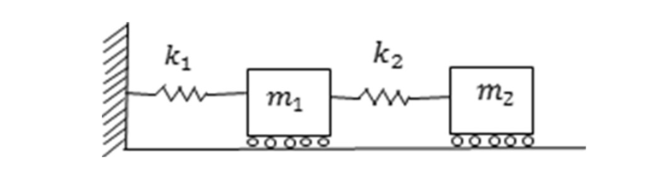
\includegraphics[width=\columnwidth]{figs/g54.fig1.png}
    \caption{ }
    \label{}
\end{figure}                   
\\    \hfill{GATE NM 2022} \\

\solution

\begin{figure}[h]
    \centering
    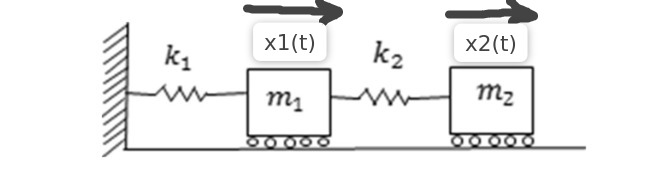
\includegraphics[width=\columnwidth]{figs/g54.fig2.jpeg}
    \caption{ }
    \label{}
\end{figure} 

\begin{align}
m_2\ddot{x_2}(t) + k_2\brak{\ddot{x_2}(t)-\ddot{x_1}(t)}&=0 \\
m_1\ddot{x_1}(t) + k_2\brak{\ddot{x_2}(t)-\ddot{x_1}(t)}+ k_1\ddot{x_1}(t)&=0
\end{align}

\begin{align}
\ddot{x_1}(t) + x_2(t) &=0 
\label{eq:ishitha.g22.nm.54.1.eq}\\
\ddot{x_2}(t) + 2\brak{x_2(t)-x_1(t)} &= 0 
\label{eq:ishitha.g22.nm.54.2.eq}
\end{align}

Substituting  ~\eqref{eq:ishitha.g22.nm.54.1.eq} in  ~\eqref{eq:ishitha.g22.nm.54.2.eq}
\begin{align}
\ddddot{x_1}(t) + 2\ddot{x_1}(t) + x_1(t) &= 0 
\label{eq:ishitha.g22.nm.54.3.eq}
\end{align}

Applying Laplace transform on both sides of ~\eqref{eq:ishitha.g22.nm.54.3.eq}
\begin{align}
\mathcal{L}\brak{\ddddot{x_1}(t) + 2\ddot{x_1}(t) + x_1(t)} &= 0 \\
X_1(s)\brak{s^4 - s^3 x_1(0) - s^2 \dot{x_1}(0) -s\ddot{x_1}(0)-\dddot{x_1}(0)} &+\nonumber \\ 2X_1(s)\brak{s^2-sx_1(0)-\dot{x_1}(0)} + X_1(s) =0
\end{align}
let $x_1(t)$ be constant at t=0
\begin{align}
X_1(s)\brak{s^4 - s^3 x_1(0) - s^2 \dot{x_1}(0)} &+\nonumber \\ 2X_1(s)\brak{s^2-sx_1(0)} + X_1(s) =0\\
X_1(s)\brak{s^4 -\brak{s^3+2s}x_1(0) - s^2 \brak{\dot{x_1}(0)-2}  +1}&=0
\end{align}

\end{document}
